\chapter{Problem Statement and Background}

In this chapter, we will state and formalize the problem statement and discuss the background information required to properly understand the solution proposed for the problem statement.

\section{Problem Statement}

In this section, we will formalize the problem statement and go over some use cases for our solution. Over the past decade, there has been widespread adoption of virtual reality with consumer-grade virtual reality headsets, such as the Oculus Rift, the HTC Vive, and more recently the Apple Vision Pro, immersive gaming and virtual worlds where you can move around. Some of these applications need to know the exact position of the user as they move around. There are a few ways in which the exact position of the user can be found. One could use trackers placed on the user along with the sensor. Another way could be to use multiple cameras, placed at different locations, looking at the same view from different angles; the position of the person in multiple cameras, along with the information of the position of the cameras, can be used to find the position of the person in consideration.\newline

All the existing methods require pre-preparation of some kind to some extent, be they either placing a sensor or using multiple cameras, along with the pre-preparation. The methods also need a lot of equipment to gain as much data about the scene as possible. Although the amount of data does help locate precise coordinates, it is not easy to implement, move around, or translate the implementation to other use cases.\newline

There exists a gap in the research for a method that needs no pre-preparation or a lot of specialized equipment to gather data. Through the scope of this thesis, we will propose a method to calculate the coordinates of a person/object in three-dimensional space, while limiting the data stream to monocular images from a regular RGB camera. These images inherently lack depth information apart from the context clues present in the scene such as walls, shadows, and other objects in the room being captured. Hence, the method needs to make smart use of the information that is available. The continuous use of the method over the consecutive frames of a video stream gives the change of coordinates of a person over time, allowing the method to record object positions in the room and to track them. This opens up more applications for the methods, such as tracking the trajectory of people in security video footage to account for their whereabouts in relation to everything else.

\section{Background}

We will divide this section into a few subsections, each relating to one of the sub-problems, and discuss the background information needed for them.

\subsection{Mapping The Room}

To place the person/object accurately in the room, we first need to understand the context of the scene in the image, the position of the corners, the wall, the roof, and the floor of the room. Some tools required for this task are discussed in the following sub-sections.

\subsection{Edge Detection}

It is one of the most fundamental techniques in computer vision that becomes the basis of more complex tasks. Images in computers are stored as 2-dimensional arrays with each element storing the RGB color values of the pixels that they represent. The most basic edge detection techniques use filters, which also are smaller 2-dimensional arrays to parse over the image array and manipulate the pixel values, depending on the surrounding pixels to either turn the current pixel value to 0 (black) or 1 (white). Figure \ref{fig:Edge Detection Convolution Filter} shows a Vertical Sobel Kernel used to convolute the pixel values and detect edges.\newline


\begin{figure}[H]
    \centering
        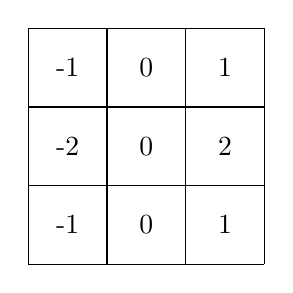
\begin{tikzpicture}
            \draw (0,0) grid (3,3);
            \node at (1-0.5,1-0.5) {-1};
            \node at (1-0.5,2-0.5) {-2};
            \node at (1-0.5,3-0.5) {-1};
            \node at (2-0.5,1-0.5) {0};
            \node at (2-0.5,2-0.5) {0};
            \node at (2-0.5,3-0.5) {0};
            \node at (3-0.5,1-0.5) {1};
            \node at (3-0.5,2-0.5) {2};
            \node at (3-0.5,3-0.5) {1};
        \end{tikzpicture}
    \caption{Edge Detection Convolution Filter}
    \label{fig:Edge Detection Convolution Filter}
\end{figure}



Once the filter is done parsing the image, all the edges are represented by white pixels and everything else is black. More sophisticated techniques like Canny edge detection combine the convolutions step with other steps to find the edges. \ref{fig: Test Room Image} shows the original image and \ref{fig: Test Room Post processed through the Canny edge detector} shows the result obtained after the image is processed through the Canny edge detector.

\begin{figure}[H]
    \centering
    \includegraphics[width=0.8\textwidth]{yo.png}
    \caption{Test Room Image}
    \label{fig: Test Room Image}
\end{figure}

\begin{figure}[H]
    \centering
    \includegraphics[width=0.8\textwidth]{white_edge.png}
    \caption{Test Room Post processed through the Canny edge detector}
    \label{fig: Test Room Post processed through the Canny edge detector}
\end{figure}


\subsection{Line detection}

Line detection is one of the techniques that uses edge detection as its basis, with other techniques built over the edge detection to find the equations of the lines that the edges represent Advanced methods such as Generalized Hough transform can even detect complex shapes like circles, or ellipses. \ref{fig: Test Room Processed through Standard Hough Transform} shows the line detected in \ref{fig:Edge Detection Convolution Filter} by one of the more basic methods called the Standard Hough Transform.

\begin{figure}[H]
    \centering
    \includegraphics[width=0.8\textwidth]{white_lines.png}
    \caption{Test Room Processed through Standard Hough Transform}
    \label{fig: Test Room Processed through Standard Hough Transform}
\end{figure}

\subsection{Corner detection}

Corner detection is one of the more advanced techniques in computer vision that uses both line and edge detection to find intersection points of edges that also have extreme gradient changes or color changes in multiple directions. \ref{fig: Test Room Processed through Harris Corner Detector} shows all the detected corners in one by using the Harris Corner Detector.

\begin{figure}[H]
    \centering
    \includegraphics[width=0.8\textwidth]{white_corners.png}
    \caption{Test Room Processed through Harris Corner Detector}
    \label{fig: Test Room Processed through Harris Corner Detector}
\end{figure}

\subsection{Image segmentation}

Image segmentation is one of the more advanced computer vision techniques, used to find different regions of an image, using multiple steps and methods. The idea is to start with a seed pixel and grow the region based on neighboring pixels. Segmentation works particularly well when used in combination with deep learning techniques, like neural networks.

\subsection{Person/object detection }

Effectively tracking the trajectory of a person within an input video necessitates the continuous detection of the person in each frame and the maintenance of coordinates. Although tracking coordinates in a general image space poses minimal challenges, the transfer of these coordinates to a 3-D space introduces complexities. Tackling this task is the main objective of this thesis. However, the first step is to move forward in this problem to effectively detect the person/object that will be the main focus in the frame. Neural networks are the most advanced computational models currently available to do this task.

\subsubsection{Neural networks}

Neural networks are very versatile, and complex computational models with various applications and implementations. Computational neural networks are artificially created structures that essentially are supposed to mimic biological neural networks. They consist of nodes and connections. The nodes are supposed to represent the neurons, and the edges represent the connections between the neurons. A neural network while mimicking a biological neural network has the structure of a weighted directed graph. A neural network can have a simple linear structure or a very complex structure. However, the information always flows forward like it does in a directed graph.\newline

A simple neural network contains layers of neurons and each layer is completely connected to the next. Each neuron (node) depending on the type of the neural network takes a {0}, {1} value or value between [0,1]. This number is called the activation of the neuron and represents how active the neuron is. That is how much it contributes to the next layer. The activation of the neuron in combination with the weight of the new edge between the node and the next node past trough function called the activation function, and determines how active the next node will be.\newline


\begin{figure}[h]
    \centering
    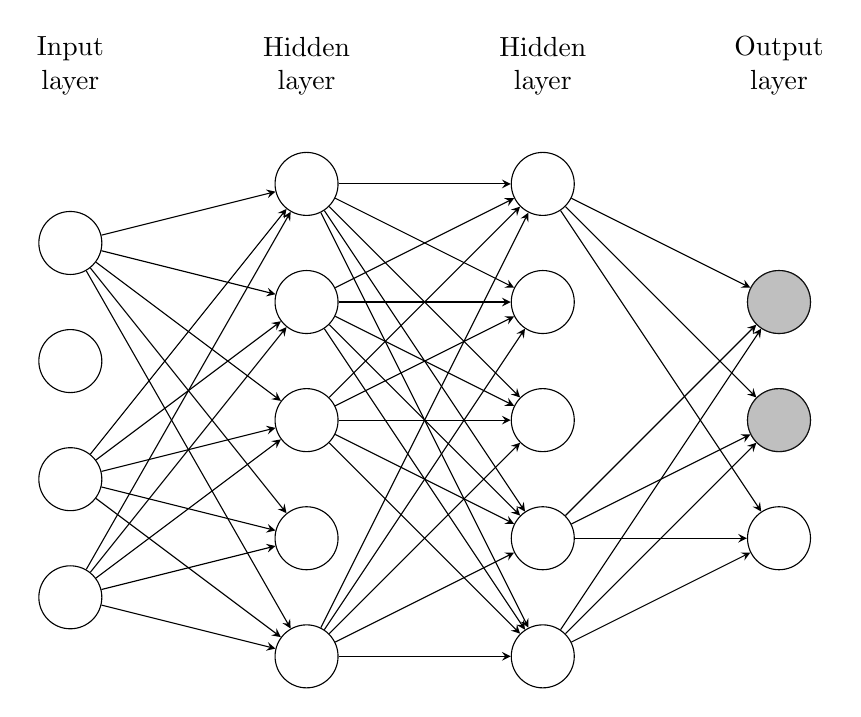
\begin{tikzpicture}[x=1.5cm, y=1.5cm, >=stealth, node distance=2.5cm]
        % Define node style
        \tikzstyle{neuron}=[circle,draw=black,minimum size=8mm]
        
        % Input layer nodes
        \foreach \m/\l [count=\y] in {1,2,3,4}
            \node [neuron] (input-\m) at (-2,2-\y) {};
            
        %Hidden layer nodes
        \foreach \m/\l [count=\y] in {1,2,3,4,5}
            \node [neuron] (hidden1-\m) at (0,2.5-\y) {};
        
        % Second hidden layer nodes
        \foreach \m [count=\y] in {1,2,3,4,5}
            \node [neuron] (hidden2-\m) at (2,2.5-\y) {};
        
        % Output layer nodes
        \foreach \m [count=\y] in {1,2,3}
            \node [neuron] (output-\m) at (4,1.5-\y) {};
        
        \foreach \m [count=\y] in {1,2}
            \node [neuron, fill=black!50, opacity=0.5] (output-\m) at (4,1.5-\y) {};
        
        % Connect input layer with first hidden layer
        \foreach \l [count=\i] in {1,3,4}
            \foreach \j in {1,2,3,4,5}
                \draw [->] (input-\l) -- (hidden1-\j);
        
        % Connect first hidden layer with second hidden layer
        \foreach \l [count=\i] in {1,2,3,5}
            \foreach \j in {1,2,3,4,5}
                \draw [->] (hidden1-\l) -- (hidden2-\j);

        % Connect second hidden layer with output layer
        \foreach \l [count=\i] in {1,4,5}
            \foreach \j in {1,2,3}
                \draw [->] (hidden2-\l) -- (output-\j);

        % Annotate input layer
        \node[align=center] at (-2, 2.5) {Input\\layer};
        
        % Annotate first hidden layer
        \node[align=center] at (0, 2.5) {Hidden\\layer};
        
        % Annotate second hidden layer
        \node[align=center] at (2, 2.5) {Hidden\\layer};
        
        % Annotate output layer
        \node[align=center] at (4, 2.5) {Output\\layer};
    \end{tikzpicture}
    \caption{Neural Network Architecture with Two Hidden Layers}
    \label{fig: Neural Network Architecture with Two Hidden Layers}
\end{figure}

\ref{fig: Neural Network Architecture with Two Hidden Layers} shows a rather simple neural network. Each node is connected to every node in the next layer. Only the active edges are shown.
Any node that does not have a connection going out of it is inactive. The nodes with a black hue represent the output of the network.\newline

\subsubsection{Pose detection}

Knowing the orientation that the person is in (sitting, standing, etc.) is particularly important to accurately find the place where they are interacting with the ground plane, especially in cases where the person is occluded by other objects or is only partially visible in the image space. This can be done by using the proportions of the human body and extending the visible part of the person, according to human body proportions. Google has worked on this and has a tool called Google Media Pipeline \cite{12} which is used in the implementation phase of the solution discussed in the following chapters. 

\subsubsection{Perspective views}

The 3-dimensional world, when projected on a 2-dimensional image space, forms of perspective, projection, also known as a perspective view. A perspective view is the most accurate representation of how the 3-dimensional world appears from a particular viewpoint. Perspective views are commonly used in computer graphics and engineering to showcase realistic depictions of 3-dimensional objects and scenes. They are often used to render the world in virtual and augmented reality. All images captured by a camera also exist in perspective views. The videos/images obtained from a camera can be in one of three perspectives depending on the orientation of the camera to the surrounding world. The perspectives include one vanishing point, two vanishing points, or three vanishing points perspective view. A vanishing point is an imaginary point in the image plane through which all receding parallel lines converge or appear to converge. For each plane in the view that is not orthogonal to the viewing plane, there exists a vanishing point. Consider being in a cubical room, standing in the centroid of the floor in such a way that you are directly facing the centroid of one of the walls. The view obtained as shown in Figure 3-7 would be one vanishing point perspective view.\newline

\begin{figure}[H]
    \centering
    \includegraphics[width=0.9\textwidth]{1vp view.PNG}
    \caption{One Vanishing point perspective view}
    \label{fig: One Vanishing point perspective view}
\end{figure}

Now if you rotate to face one of the edges between two walls, the view obtained as shown in \ref{fig: Two Vanishing point perspective view} would be two vanishing point perspective view.\newline

\begin{figure}[H]
    \centering
    \includegraphics[width=0.9\textwidth]{2vp view.PNG}
    \caption{Two Vanishing point perspective view}
    \label{fig: Two Vanishing point perspective view}
\end{figure}


Further, if you lift your head to look at the corner, the view obtained would be as shown in \ref{fig: Three vanishing point perspective view} to be three vanishing point perspective view.\newline

\begin{figure}[H]
    \centering
    \includegraphics[width=0.9\textwidth]{3vp view.PNG}
    \caption{Three vanishing point perspective view}
    \label{fig: Three vanishing point perspective view}
\end{figure}


\subsection{Tracking}

The task of following an object or a person through a video stream is known as tracking. In more formal terms, it can be stated, as keeping track of a subject whether it is an object or a person through a video stream, as they move through the field of view. Since videos are nothing but consecutive images, finding the coordinates of the person/object through all of the images and presenting the change in them with the change in time yields the trajectory of the subject, essentially tracking them. However, looking for the subject in the entire image space is a computationally expensive task and can be made much cheaper to do so. Some techniques that will be used in the next section are discussed as follows.

\subsubsection{Predictive processing}

Making predictions for the future based on the current understanding of the world, and the physics of it is called predictive processing. Living beings constantly use predictive processing to better interact with the dynamic world around them. 

\subsubsection{Feedback mechanism}

Constant input to tweak and change the current strategy used to complete a task is called a feedback mechanism.
